%ATRACTOR DE LORENZ
El sistema de ecuaciones de Lorenz es un ejemplo de un sistema de ecuaciones diferenciales de orden 1, tridimensional, no lineal, que tiene un comportamiento caótico para algunos valores de sus parámetros. Este sistema de ecuaciones permite modelar los rollos de convección que se producen en la atmosfera terrestre. Es un modelo simplificado de la convección de Rayleigh-Benard (ecuaciones de Navier-Stokes con hipótesis de Boussinesq).
\begin{equation}
\left\{ 
\begin{matrix}
dx/dt =& Pr (y(t) - x(yt)) \\
dy/dt =& Ra x(t) - y(t) - x(t)z(t) \\
dz/dt =& x(t) y(t) - \beta z(t)
\end{matrix} \right.
\end{equation}
Donde $Pr$ es el número de Prandtl y $Ra$ es el número de Rayleigh. Las variables dinámicas $x$, $y$ y $z$ represetan el estado del sistema a cada instante $t$:

\begin{itemize}
\item x(t) es proporcional a la intensidad del movimiento de convección  
\item y(t) es proporcional a la diferencia de temperatura entre las corrientes ascendentes y descendentes
\item z(t) es proporcional a la diferencia entre el perfil vertical de temperatura y un perfil vertical de temperatura lineal
\end{itemize}

Los sistemas dinámicos son sistemas que son función del tiempo. Que sea caótico significa que varia de manera no lineal y a su vez que el sistema presenta sensibilidad a frente a los parámetros entrada. Además presentan un comportamiento oscilante, pudiendo ser periodico o no periodico. \\

\subsubsection{Parte 1}
Las Figuras \ref{lorenz1} y \ref{lorenz2} reproducen los gráficos del articulo \textit{Deterministic Nonperiodic Flow} de Lorenz
\begin{figure} [H]
\begin{center}
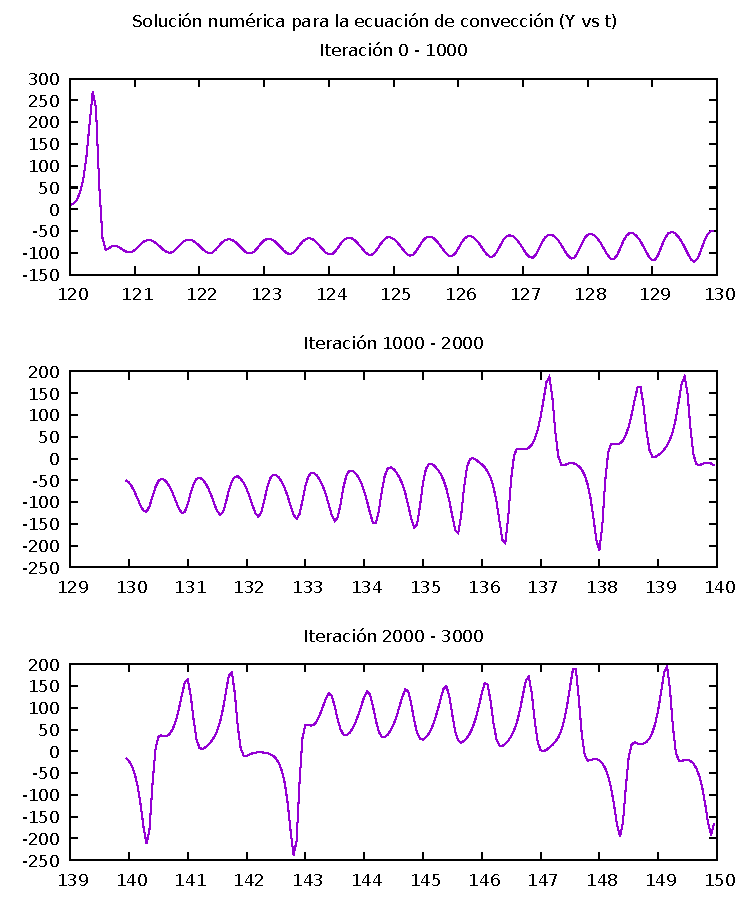
\includegraphics[width=0.8\textwidth]{./parte4/graficos/FIGURA1.pdf}
\caption{} \label{lorenz1}
\end{center}
\end{figure}

\begin{figure} [H]
\begin{center}
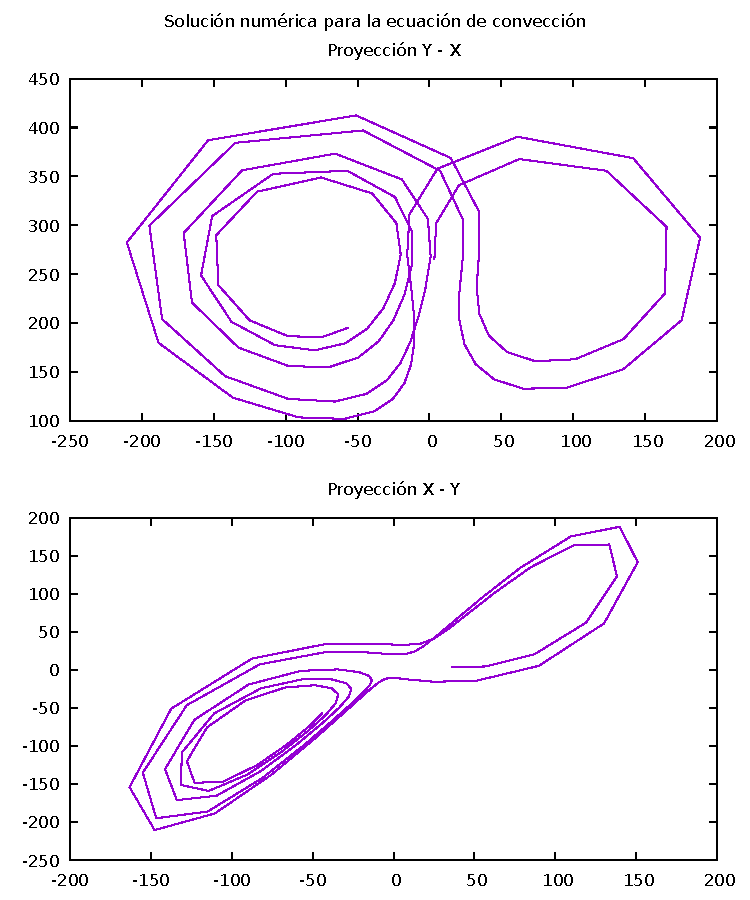
\includegraphics[width=0.8\textwidth]{./parte4/graficos/FIGURA2.pdf}
\caption{} \label{lorenz2}
\end{center}
\end{figure}

%---------------------------

\subsubsection{Parte 2}

Se grafica la solución a la ecuación de convección utilizando los siguientes valores: $Pr=10$, $\beta= 8/3$ y $Ra = 0.5 \, , \, 10 , \, 28$ 

\begin{figure} [H]
\begin{center}
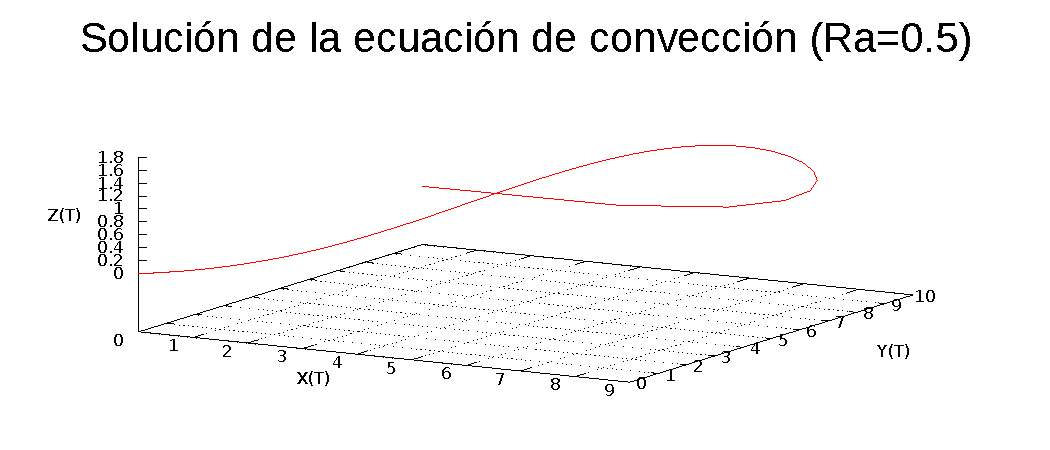
\includegraphics[width=0.8\textwidth]{./parte4/graficos/grafico_P3_3d_ra05.pdf}
\caption{}
\end{center}
\end{figure}

\begin{figure} [H]
\begin{center}
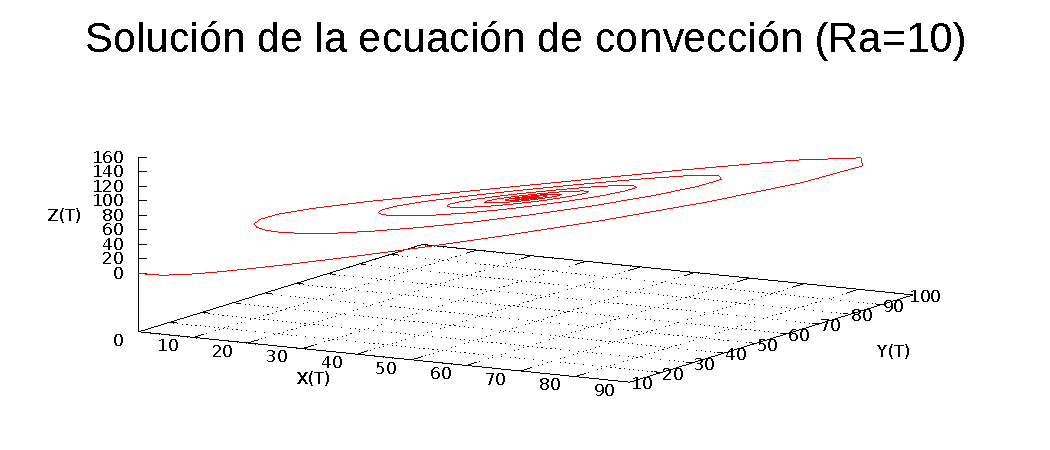
\includegraphics[width=0.8\textwidth]{./parte4/graficos/grafico_P3_3d_ra10.pdf}
\caption{}
\end{center}
\end{figure}

\begin{figure} [H]
\begin{center}
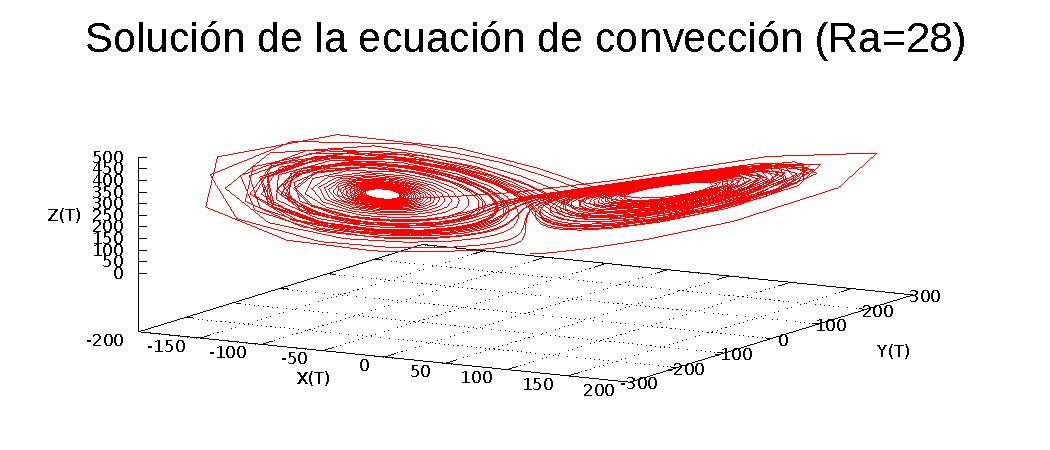
\includegraphics[width=0.8\textwidth]{./parte4/graficos/grafico_P3_3d_ra28.pdf}
\caption{}
\end{center}
\end{figure}

%---------------------------

\subsubsection{Parte 3}
Haciendo variar paulatinamente $Ra$ entre 0 y 30

\begin{figure} [H]
\hspace{-1cm} 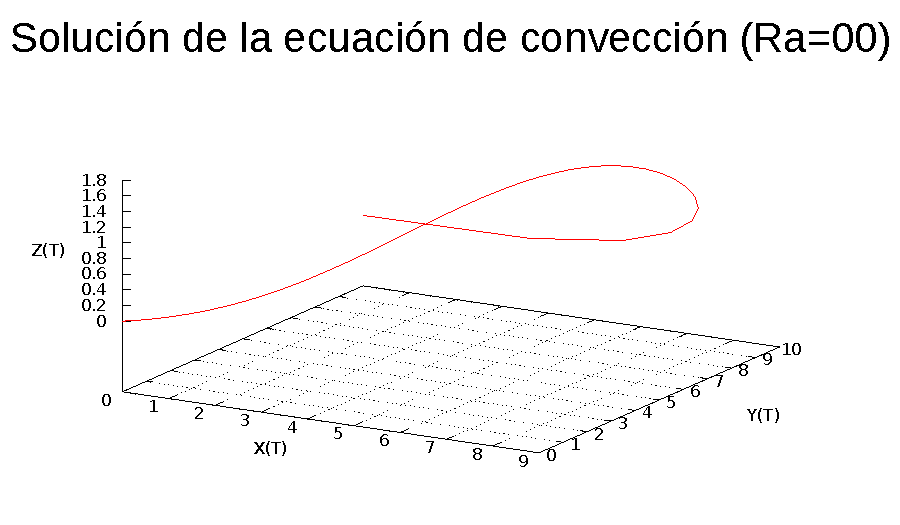
\includegraphics[width=0.6\textwidth]{./parte4/graficos/grafico_P3_3d_ra00.pdf}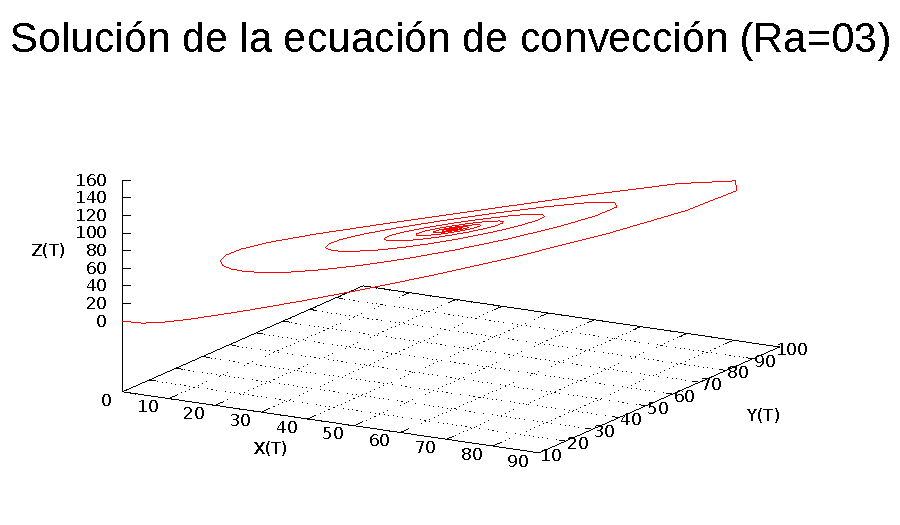
\includegraphics[width=0.6\textwidth]{./parte4/graficos/grafico_P3_3d_ra03.pdf}
\caption{} 
\end{figure}

\begin{figure} [H]
\hspace{-1cm} 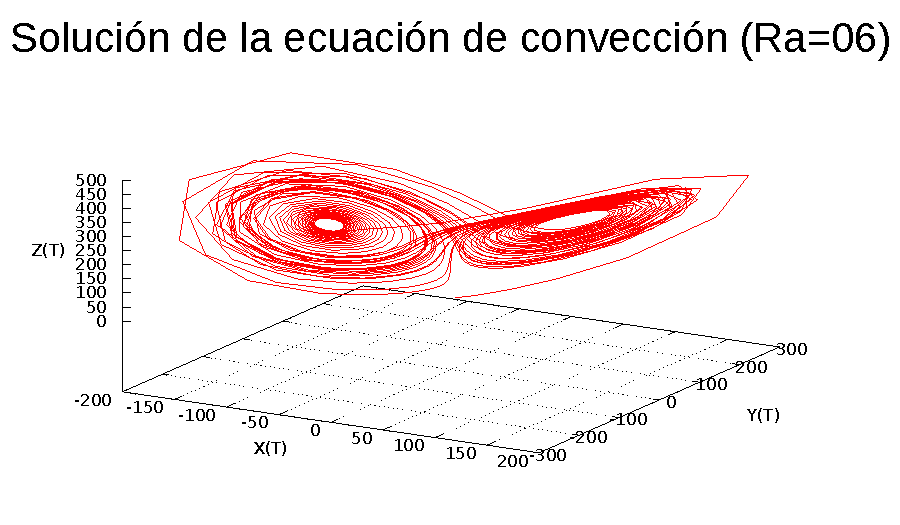
\includegraphics[width=0.6\textwidth]{./parte4/graficos/grafico_P3_3d_ra06.pdf}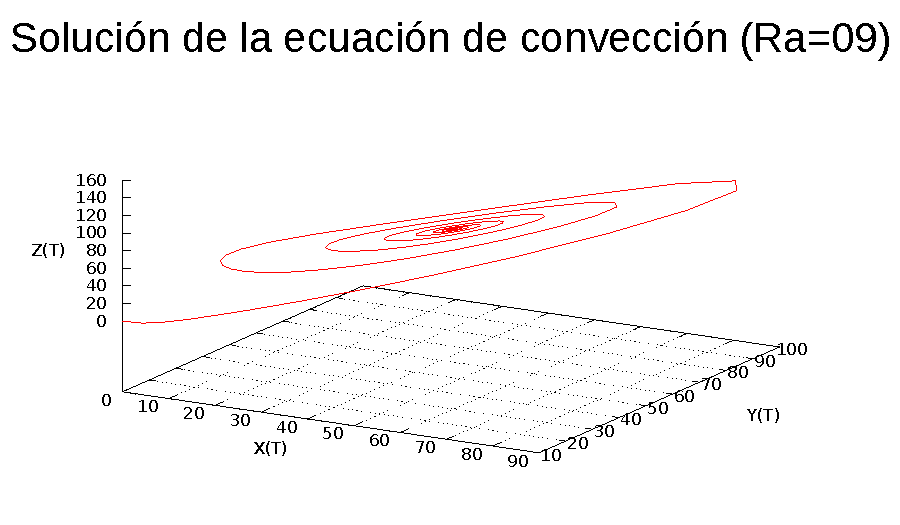
\includegraphics[width=0.6\textwidth]{./parte4/graficos/grafico_P3_3d_ra09.pdf}
\caption{} 
\end{figure}

\begin{figure} [H]
\hspace{-1cm} 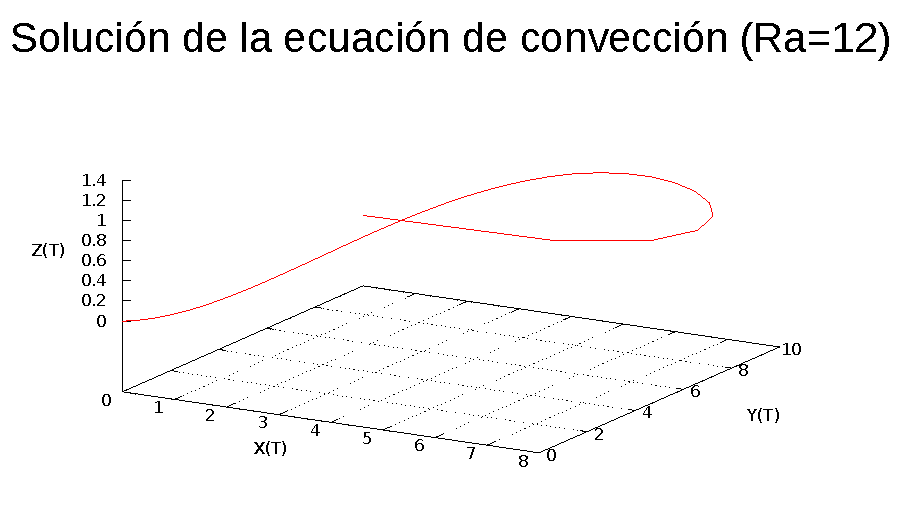
\includegraphics[width=0.6\textwidth]{./parte4/graficos/grafico_P3_3d_ra12.pdf}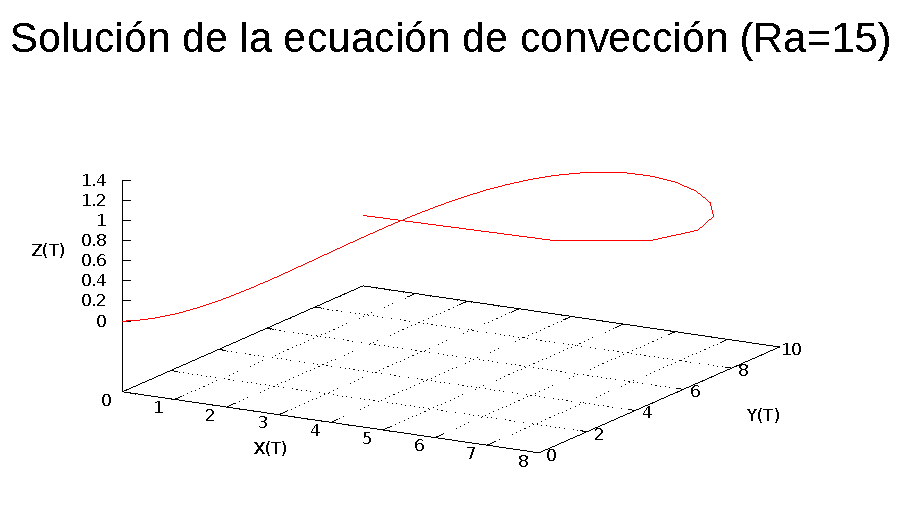
\includegraphics[width=0.6\textwidth]{./parte4/graficos/grafico_P3_3d_ra15.pdf}
\caption{} 
\end{figure}

\begin{figure} [H]
\hspace{-1cm} 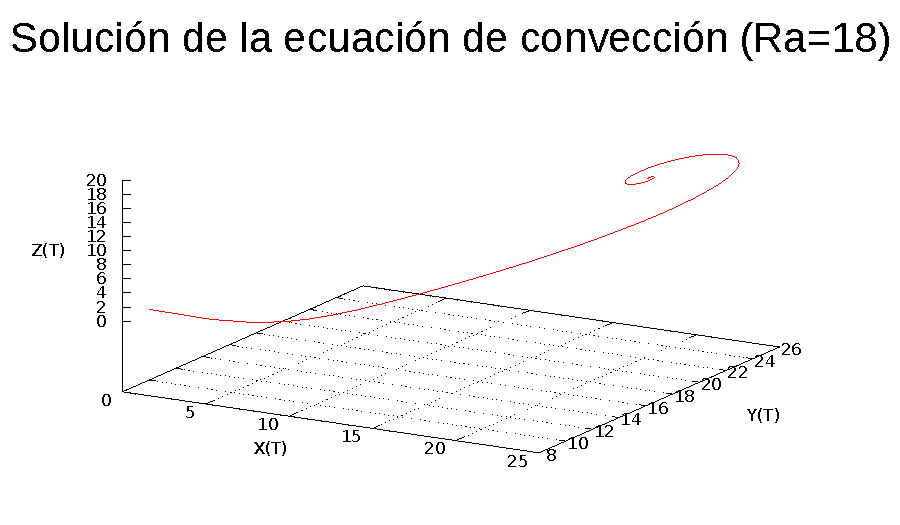
\includegraphics[width=0.6\textwidth]{./parte4/graficos/grafico_P3_3d_ra18.pdf}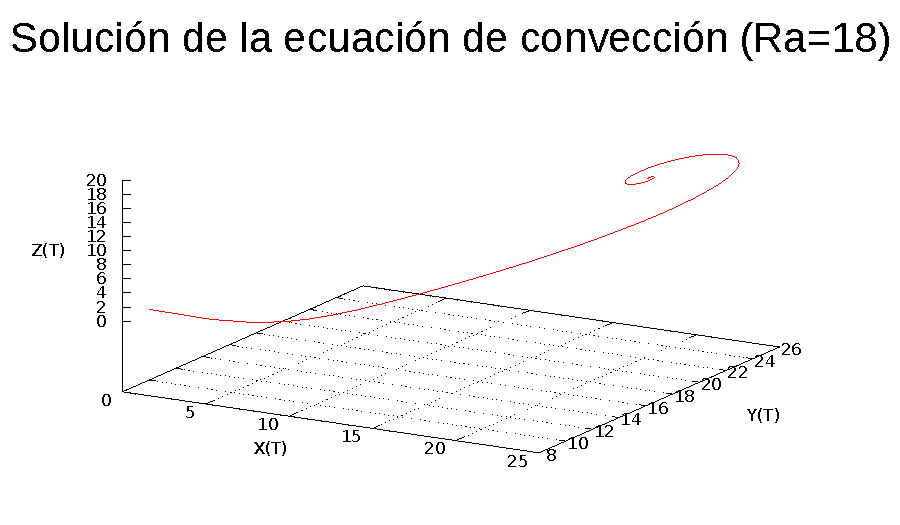
\includegraphics[width=0.6\textwidth]{./parte4/graficos/grafico_P3_3d_ra18.pdf}
\caption{} 
\end{figure}

\begin{figure} [H]
\hspace{-1cm} 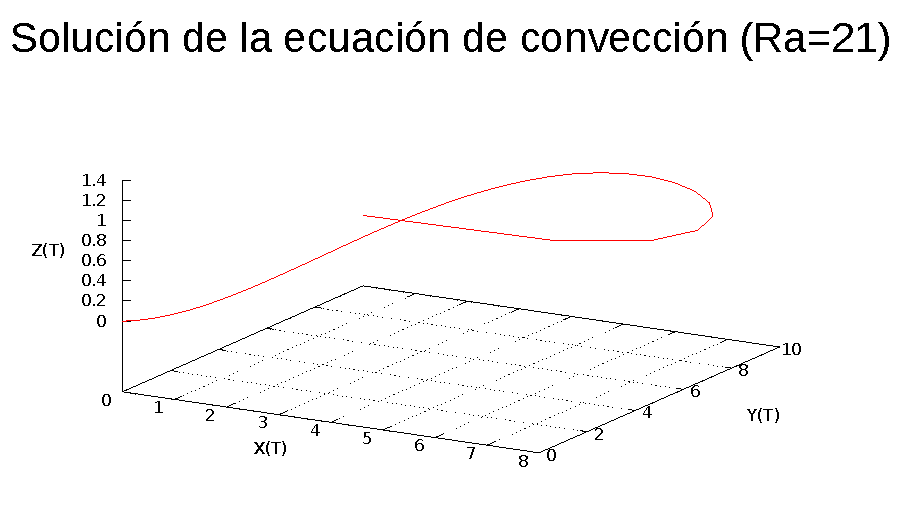
\includegraphics[width=0.6\textwidth]{./parte4/graficos/grafico_P3_3d_ra21.pdf}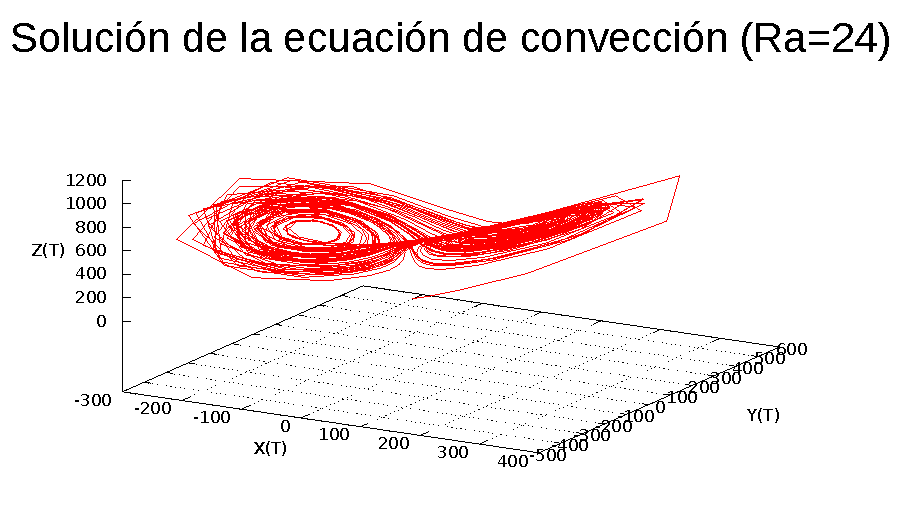
\includegraphics[width=0.6\textwidth]{./parte4/graficos/grafico_P3_3d_ra24.pdf}
\caption{} 
\end{figure}

\begin{figure} [H]
\hspace{-1cm} 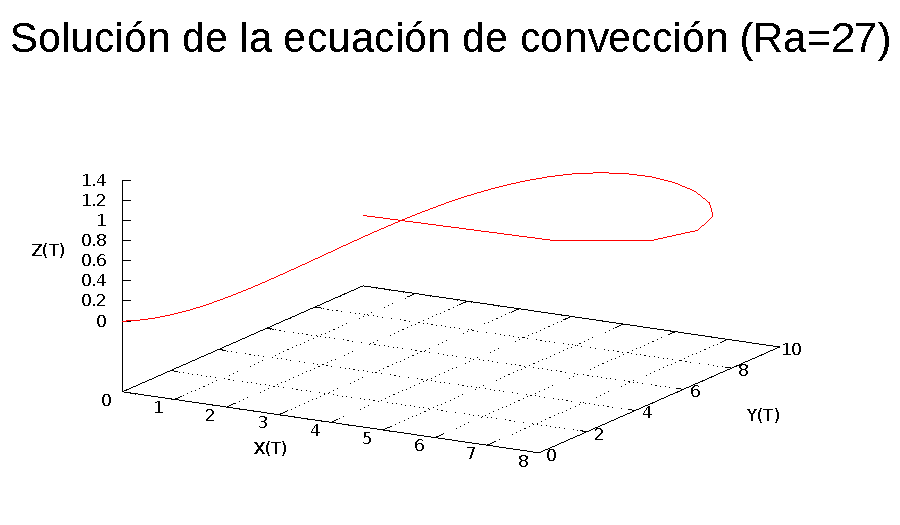
\includegraphics[width=0.6\textwidth]{./parte4/graficos/grafico_P3_3d_ra27.pdf}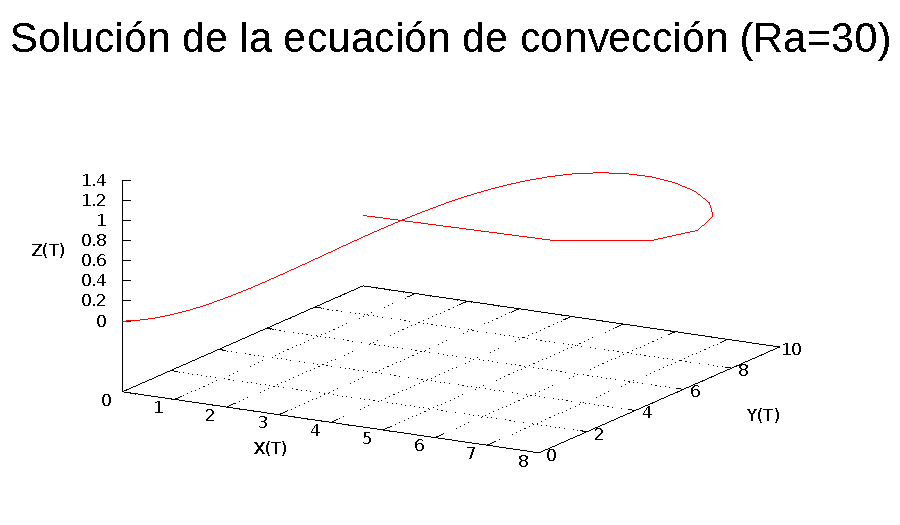
\includegraphics[width=0.6\textwidth]{./parte4/graficos/grafico_P3_3d_ra30.pdf}
\caption{} 
\end{figure}